\documentclass[8pt,aspectratio=169]{beamer}
\usetheme{Madrid}
\usepackage{graphicx}
\usepackage{amsmath}
\usepackage{amssymb}
\usepackage{tikz}
\usepackage{tcolorbox}

% Color definitions (Madrid theme with lavender)
\definecolor{mlblue}{RGB}{0,102,204}
\definecolor{mlpurple}{RGB}{51,51,178}
\definecolor{mllavender}{RGB}{173,173,224}
\definecolor{mllavender2}{RGB}{193,193,232}
\definecolor{mllavender3}{RGB}{204,204,235}
\definecolor{mllavender4}{RGB}{214,214,239}
\definecolor{mlorange}{RGB}{255, 127, 14}
\definecolor{mlgreen}{RGB}{44, 160, 44}
\definecolor{mlred}{RGB}{214, 39, 40}

% Apply custom colors to Madrid theme
\setbeamercolor{palette primary}{bg=mllavender3,fg=mlpurple}
\setbeamercolor{palette secondary}{bg=mllavender2,fg=mlpurple}
\setbeamercolor{palette tertiary}{bg=mllavender,fg=white}
\setbeamercolor{palette quaternary}{bg=mlpurple,fg=white}
\setbeamercolor{structure}{fg=mlpurple}
\setbeamercolor{frametitle}{fg=mlpurple,bg=mllavender3}

% Remove navigation symbols
\setbeamertemplate{navigation symbols}{}

% Math commands
\newcommand{\given}{\mid}

% BSc Pedagogical boxes
\newtcolorbox{checkpoint}[1][]{
    colback=yellow!10!white,
    colframe=yellow!75!black,
    title=\textbf{Checkpoint: #1},
    fonttitle=\bfseries,
    left=3pt, right=3pt, top=3pt, bottom=3pt
}

\newtcolorbox{intuition}[1][]{
    colback=purple!5!white,
    colframe=purple!75!black,
    title=\textbf{Intuition: #1},
    fonttitle=\bfseries,
    left=3pt, right=3pt, top=3pt, bottom=3pt
}

\newtcolorbox{realworld}[1][]{
    colback=orange!5!white,
    colframe=orange!75!black,
    title=\textbf{Real World: #1},
    fonttitle=\bfseries,
    left=3pt, right=3pt, top=3pt, bottom=3pt
}

% Bottom annotation command
\newcommand{\bottomnote}[1]{%
\vfill
\vspace{-2mm}
\textcolor{mllavender2}{\rule{\textwidth}{0.4pt}}
\vspace{1mm}
\footnotesize
\textbf{#1}
}

% Title information
\title{Recurrent Neural Networks}
\subtitle{Discovery-Based Introduction to Sequential Learning}
\author{}
\date{}

\begin{document}

% ==================== ACT 1: THE CHALLENGE ====================

% Slide 1: Title
\begin{frame}[plain]
    \titlepage
\end{frame}

% Slide 2: Discovery Question - Thought Experiment
\begin{frame}{Before We Begin: A Thought Experiment}
    \begin{center}
    \textbf{\Large Imagine You're Building a Text Prediction System}
    \end{center}

    \vspace{1em}
    \begin{columns}[T]
        \begin{column}{0.55\textwidth}
            \textbf{Your Challenge:}

            Given text: ``The weather today is very''

            Your system must predict: ``\textcolor{mlgreen}{sunny}'' or ``\textcolor{mlgreen}{nice}''

            \vspace{1em}
            \textbf{Design Questions:}
            \begin{enumerate}
                \item How much previous text should you look at?
                \item What if the text is 100 words long?
                \item How do you remember important words from earlier?
                \item What makes ``weather'' more important than ``is''?
            \end{enumerate}

            \vspace{1em}
            \colorbox{orange!10}{\parbox{0.95\columnwidth}{
                \textbf{Key Insight:} To predict well, you need to \textit{remember} what came before. But how much? And for how long?
            }}
        \end{column}

        \begin{column}{0.43\textwidth}
            \textbf{Your Design:}

            \vspace{0.5em}
            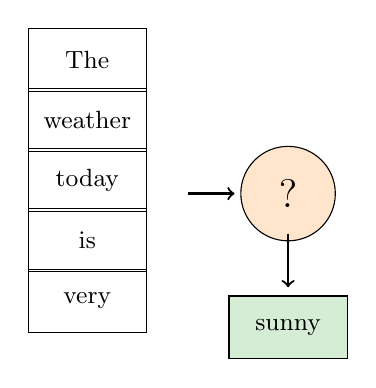
\begin{tikzpicture}[scale=0.85, every node/.style={font=\small}]
                % Input boxes
                \foreach \i/\word in {0/The, 1/weather, 2/today, 3/is, 4/very} {
                    \node[draw, rectangle, minimum width=1.5cm, minimum height=0.8cm] at (0, -\i*0.9) {\word};
                }

                % Question mark for memory
                \node[draw, circle, fill=orange!20, minimum size=1.2cm] at (3, -2) {\Large ?};

                % Output
                \node[draw, rectangle, fill=mlgreen!20, minimum width=1.5cm, minimum height=0.8cm] at (3, -4) {sunny};

                % Arrow
                \draw[->, thick] (1.5, -2) -- (2.2, -2);
                \draw[->, thick] (3, -2.6) -- (3, -3.4);
            \end{tikzpicture}

            \vspace{1em}
            \textbf{What should go in the ``?'' box?}
        \end{column}
    \end{columns}

    \bottomnote{Next slide reveals: What neural networks are actually trying to do}
\end{frame}

% Slide 3: What Is This About?
\begin{frame}{What Is This About?}
    \begin{center}
    \textbf{\Large The Core Task: Predict the Next Word}
    \end{center}

    \vspace{1em}
    \begin{columns}[T]
        \begin{column}{0.48\textwidth}
            \textbf{The Prediction Challenge:}

            \vspace{0.5em}
            \textbf{Example 1:} Short Context

            Input: ``My name is''

            Prediction: ``\textcolor{mlgreen}{John}'' or ``\textcolor{mlgreen}{Sarah}''

            \textcolor{gray}{(Need to remember: 2-3 words)}

            \vspace{1em}
            \textbf{Example 2:} Medium Context

            Input: ``The cat that ate the fish''

            Prediction: ``\textcolor{mlgreen}{was}'' (singular verb!)

            \textcolor{gray}{(Need to remember: ``cat'' is singular, 5 words back)}

            \vspace{1em}
            \textbf{Example 3:} Long Context

            Input: ``In 1492, Columbus sailed across the Atlantic Ocean and discovered America. This voyage changed''

            Prediction: ``\textcolor{mlgreen}{history}'' or ``\textcolor{mlgreen}{everything}''

            \textcolor{gray}{(Need to remember: entire story, 15+ words)}
        \end{column}

        \begin{column}{0.48\textwidth}
            \begin{intuition}[Why This Matters]
            If we can predict the next word:
            \begin{itemize}
                \item \textbf{Autocomplete:} ``Did you mean\ldots?''
                \item \textbf{Translation:} Convert word-by-word
                \item \textbf{Chatbots:} Generate responses
                \item \textbf{Search:} Understand queries
            \end{itemize}
            \end{intuition}

            \vspace{1em}
            \textbf{The Memory Problem:}

            \begin{center}
            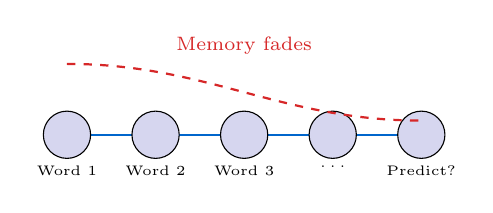
\begin{tikzpicture}[scale=0.9]
                % Memory span visualization
                \draw[thick, mlblue] (0,0) -- (5,0);
                \node[circle, draw, fill=mllavender4, minimum size=0.6cm] at (0, 0) {};
                \node[below, font=\tiny] at (0, -0.3) {Word 1};

                \node[circle, draw, fill=mllavender4, minimum size=0.6cm] at (1.25, 0) {};
                \node[below, font=\tiny] at (1.25, -0.3) {Word 2};

                \node[circle, draw, fill=mllavender4, minimum size=0.6cm] at (2.5, 0) {};
                \node[below, font=\tiny] at (2.5, -0.3) {Word 3};

                \node[circle, draw, fill=mllavender4, minimum size=0.6cm] at (3.75, 0) {};
                \node[below, font=\tiny] at (3.75, -0.3) {$\ldots$};

                \node[circle, draw, fill=mllavender4, minimum size=0.6cm] at (5, 0) {};
                \node[below, font=\tiny] at (5, -0.3) {Predict?};

                % Memory fade
                \draw[thick, mlred, dashed] (0, 1) to[out=0, in=180] (5, 0.2);
                \node[above, mlred, font=\scriptsize] at (2.5, 1) {Memory fades};
            \end{tikzpicture}
            \end{center}

            \textbf{Question:} How far back can we remember?
        \end{column}
    \end{columns}

    \bottomnote{Every word depends on context - but how much context can we handle?}
\end{frame}

% Slide 4: Sequential Data Examples
\begin{frame}{Why Context Matters: Real Examples}
    \begin{columns}[T]
        \begin{column}{0.48\textwidth}
            \textbf{Example 1: Grammar Rules}

            \vspace{0.5em}
            ``The \textcolor{mlblue}{cat} is sleeping''

            $\rightarrow$ Predict: ``\textcolor{mlgreen}{purring}'' (cat action)

            \vspace{0.3em}
            ``The \textcolor{mlblue}{dog} is sleeping''

            $\rightarrow$ Predict: ``\textcolor{mlgreen}{snoring}'' (dog action)

            \textbf{Insight:} Need to remember the subject!

            \vspace{1em}
            \textbf{Example 2: Names}

            \vspace{0.5em}
            ``J'' $\rightarrow$ ``\textcolor{mlgreen}{o}'' (could be ``Jo'')

            ``Jo'' $\rightarrow$ ``\textcolor{mlgreen}{h}'' (building ``Joh'')

            ``Joh'' $\rightarrow$ ``\textcolor{mlgreen}{n}'' (common: ``John'')

            \textbf{Insight:} Each prediction depends on ALL previous characters!

            \vspace{1em}
            \textbf{Example 3: Sentiment}

            \vspace{0.5em}
            ``This movie is'' $\rightarrow$ ``\textcolor{mlgreen}{amazing}''

            ``This movie is not'' $\rightarrow$ ``\textcolor{mlred}{amazing}''

            \textbf{Insight:} One word (``not'') flips entire meaning!
        \end{column}

        \begin{column}{0.48\textwidth}
            \textbf{Sequential Patterns Everywhere:}

            \vspace{0.5em}
            \begin{center}
            \includegraphics[width=0.9\textwidth]{../figures/rnn_applications_bsc.pdf}
            \end{center}

            \vspace{1em}
            \begin{checkpoint}[Understanding]
            \textbf{Question:} What do all these examples have in common?

            \vspace{0.3em}
            \textbf{Answer:} The \textit{order} matters! You cannot shuffle the words/letters/frames and get the same meaning.
            \end{checkpoint}

            \vspace{1em}
            \textbf{Types of Sequential Data:}
            \begin{itemize}
                \item \textbf{Text:} Words in sentences
                \item \textbf{Speech:} Sounds over time
                \item \textbf{Video:} Frames in sequence
                \item \textbf{Time series:} Stock prices, weather
                \item \textbf{DNA:} Gene sequences
            \end{itemize}
        \end{column}
    \end{columns}

    \bottomnote{Traditional neural networks process each input independently - they ignore order!}
\end{frame}

% Slide 5: Traditional Networks Fail
\begin{frame}{Traditional Neural Networks: The Fixed-Size Problem}
    \begin{columns}[T]
        \begin{column}{0.48\textwidth}
            \textbf{How Traditional Networks Work:}

            \vspace{0.5em}
            \begin{center}
            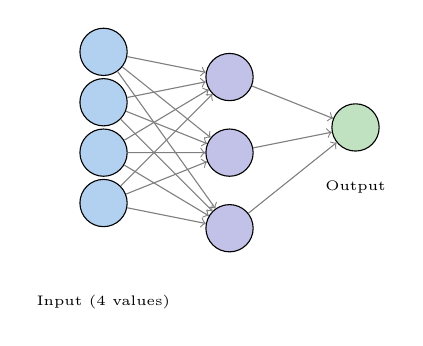
\begin{tikzpicture}[scale=0.8]
                % Input layer
                \foreach \i in {1,2,3,4} {
                    \node[circle, draw, fill=mlblue!30, minimum size=0.6cm] (i\i) at (0, -\i*0.8) {};
                }
                \node[below, font=\tiny] at (0, -4.5) {Input (4 values)};

                % Hidden layer
                \foreach \i in {1,2,3} {
                    \node[circle, draw, fill=mlpurple!30, minimum size=0.6cm] (h\i) at (2, -\i*1.2) {};
                }

                % Output layer
                \node[circle, draw, fill=mlgreen!30, minimum size=0.6cm] (o1) at (4, -2) {};
                \node[below, font=\tiny] at (4, -2.7) {Output};

                % Connections (sample)
                \foreach \i in {1,2,3,4} {
                    \foreach \j in {1,2,3} {
                        \draw[->, thin, gray] (i\i) -- (h\j);
                    }
                }
                \foreach \j in {1,2,3} {
                    \draw[->, thin, gray] (h\j) -- (o1);
                }
            \end{tikzpicture}
            \end{center}

            \textbf{Key Limitation:}
            \begin{itemize}
                \item \textcolor{mlred}{Fixed input size} (e.g., 4 numbers)
                \item \textcolor{mlred}{No memory} of previous inputs
                \item \textcolor{mlred}{Each prediction independent}
            \end{itemize}

            \vspace{1em}
            \textbf{Concrete Example:}

            Input: [0.2, 0.5, 0.1, 0.8] $\rightarrow$ Output: 0.6

            Input: [0.3, 0.4, 0.2, 0.7] $\rightarrow$ Output: 0.5

            \textcolor{gray}{Network ``forgets'' first input when processing second!}
        \end{column}

        \begin{column}{0.48\textwidth}
            \textbf{Worked Example: Text Prediction FAILS}

            \vspace{0.5em}
            Task: Predict next word after ``The cat is''

            \vspace{0.5em}
            \textbf{Attempt 1:} Use last 2 words only

            Input: ``cat is'' $\rightarrow$ Predict: ``sleeping''?

            \textcolor{mlred}{Problem:} What if sentence was ``The dog and the cat is''? Now we need 5 words!

            \vspace{1em}
            \textbf{Attempt 2:} Use last 10 words

            Input: ``\_ \_ \_ \_ \_ \_ \_ The cat is''

            (Pad with blanks if sentence is shorter)

            \textcolor{mlred}{Problems:}
            \begin{itemize}
                \item What if sentence is 50 words long?
                \item Wasted space for short sentences
                \item Still a fixed limit!
            \end{itemize}

            \vspace{1em}
            \begin{realworld}[The Real Problem]
            Natural language has \textbf{no fixed length}:
            \begin{itemize}
                \item ``Hi'' (1 word)
                \item Entire novels (100,000+ words)
            \end{itemize}

            We need \textit{variable-length} memory!
            \end{realworld}
        \end{column}
    \end{columns}

    \bottomnote{We need a network that can process ANY length sequence and remember what matters}
\end{frame}

% Slide 6: Quantify the Challenge
\begin{frame}{The Long-Range Dependency Challenge}
    \begin{columns}[T]
        \begin{column}{0.48\textwidth}
            \textbf{Challenge: Distant Information Matters}

            \vspace{0.5em}
            \textbf{Example 1:} Subject-Verb Agreement

            ``The \textcolor{mlblue}{cat} that ate the fish {\bf was} hungry''

            \textcolor{gray}{To predict ``was'' (singular), need to remember ``cat'' from 5 words ago}

            \vspace{1em}
            \textbf{Example 2:} Pronoun Resolution

            ``\textcolor{mlblue}{Sarah} went to the store. She bought milk.''

            \textcolor{gray}{``She'' refers to ``Sarah'' from previous sentence}

            \vspace{1em}
            \textbf{Example 3:} Story Coherence

            ``In 1492, Columbus discovered America.'' \\
            (50 words of other content) \\
            ``This \textcolor{mlblue}{voyage} changed history.''

            \textcolor{gray}{``Voyage'' connects to ``1492'' 50+ words earlier}

            \vspace{1em}
            \textbf{The Distance Problem:}
            \begin{itemize}
                \item Near: 1-5 words back (\textcolor{mlgreen}{Easy})
                \item Medium: 5-20 words back (\textcolor{mlorange}{Harder})
                \item Far: 20+ words back (\textcolor{mlred}{Very Hard})
            \end{itemize}
        \end{column}

        \begin{column}{0.48\textwidth}
            \textbf{Quantifying Memory Needs:}

            \vspace{0.5em}
            \begin{center}
            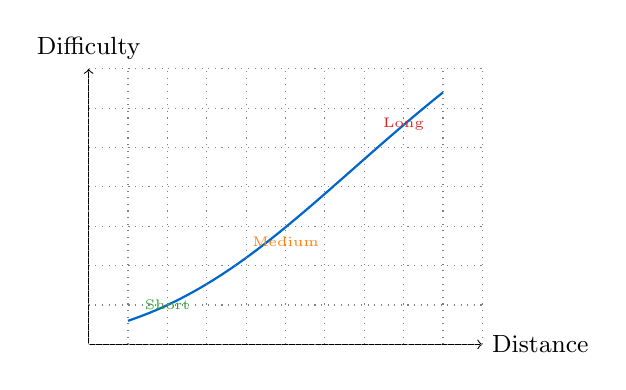
\begin{tikzpicture}[scale=1]
                % Distance vs difficulty
                \draw[->] (0,0) -- (5,0) node[right, font=\small] {Distance};
                \draw[->] (0,0) -- (0,3.5) node[above, font=\small] {Difficulty};

                % Curve showing exponential difficulty
                \draw[thick, mlblue] (0.5,0.3) .. controls (2,0.8) and (3,2) .. (4.5,3.2);

                % Annotations
                \node[mlgreen, font=\tiny] at (1, 0.5) {Short};
                \node[mlorange, font=\tiny] at (2.5, 1.3) {Medium};
                \node[mlred, font=\tiny] at (4, 2.8) {Long};

                % Grid
                \draw[dotted, gray] (0,0) grid[step=0.5] (5,3.5);
            \end{tikzpicture}
            \end{center}

            \vspace{1em}
            \textbf{Real Statistics:}
            \begin{itemize}
                \item Average sentence: 15-20 words
                \item Paragraph: 50-100 words
                \item Document: 1000+ words
            \end{itemize}

            \vspace{1em}
            \begin{checkpoint}[Key Question]
            \textbf{How do we design a network that:}
            \begin{enumerate}
                \item Handles ANY sequence length?
                \item Remembers important info from far back?
                \item Doesn't waste memory on unimportant words?
            \end{enumerate}

            \textbf{Answer:} Recurrent connections!
            \end{checkpoint}
        \end{column}
    \end{columns}

    \bottomnote{ACT 1 Summary: We need variable-length memory for sequential data - traditional networks fail}
\end{frame}

% ==================== ACT 2: FIRST SOLUTION & ITS LIMITS ====================

% Slide 7: Key Insight
\begin{frame}{The Key Insight: Memory Flowing Through Time}
    \begin{columns}[T]
        \begin{column}{0.48\textwidth}
            \textbf{The Breakthrough Idea:}

            \vspace{0.5em}
            What if the network could \textit{pass information to itself}?

            \vspace{1em}
            \textbf{Traditional Network:}

            \begin{center}
            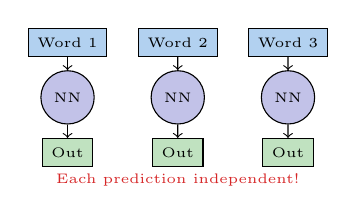
\begin{tikzpicture}[scale=0.7]
                \foreach \x/\word in {0/Word 1, 2/Word 2, 4/Word 3} {
                    \node[draw, rectangle, fill=mlblue!30] (i\x) at (\x, 1) {\tiny \word};
                    \node[draw, circle, fill=mlpurple!30] (h\x) at (\x, 0) {\tiny NN};
                    \node[draw, rectangle, fill=mlgreen!30] (o\x) at (\x, -1) {\tiny Out};
                    \draw[->] (i\x) -- (h\x);
                    \draw[->] (h\x) -- (o\x);
                }
                \node[mlred, font=\tiny] at (2, -1.5) {Each prediction independent!};
            \end{tikzpicture}
            \end{center}

            \vspace{1em}
            \textbf{Recurrent Network:}

            \begin{center}
            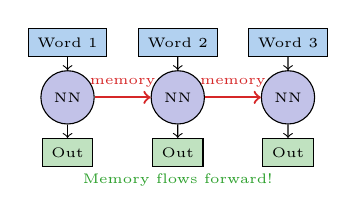
\begin{tikzpicture}[scale=0.7]
                \foreach \x/\word in {0/Word 1, 2/Word 2, 4/Word 3} {
                    \node[draw, rectangle, fill=mlblue!30] (i\x) at (\x, 1) {\tiny \word};
                    \node[draw, circle, fill=mlpurple!30] (h\x) at (\x, 0) {\tiny NN};
                    \node[draw, rectangle, fill=mlgreen!30] (o\x) at (\x, -1) {\tiny Out};
                    \draw[->] (i\x) -- (h\x);
                    \draw[->] (h\x) -- (o\x);
                }
                % Memory connections
                \draw[->, thick, mlred] (h0) -- (h2) node[midway, above, font=\tiny] {memory};
                \draw[->, thick, mlred] (h2) -- (h4) node[midway, above, font=\tiny] {memory};
                \node[mlgreen, font=\tiny] at (2, -1.5) {Memory flows forward!};
            \end{tikzpicture}
            \end{center}

            \textbf{Key Property:} Same network, reused at each time step, but with memory!
        \end{column}

        \begin{column}{0.48\textwidth}
            \begin{intuition}[Think of It Like This]
            \textbf{Traditional Network:} Goldfish memory
            \begin{itemize}
                \item Sees word
                \item Makes prediction
                \item Forgets everything
                \item Sees next word (no context!)
            \end{itemize}

            \vspace{0.5em}
            \textbf{Recurrent Network:} Taking notes
            \begin{itemize}
                \item Sees word
                \item Checks previous notes (memory)
                \item Updates notes with new info
                \item Makes prediction with full context
                \item Passes notes to next step
            \end{itemize}
            \end{intuition}

            \vspace{1em}
            \textbf{The Memory Vector:}

            Hidden state $h_t$ = ``notes'' at time $t$

            \vspace{0.5em}
            \begin{center}
            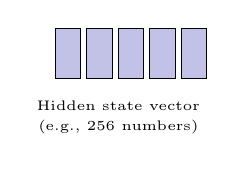
\begin{tikzpicture}[scale=0.8]
                % Hidden state vector visualization
                \foreach \i in {0,1,2,3,4} {
                    \draw[fill=mlpurple!30] (\i*0.5, 0) rectangle (\i*0.5+0.4, 0.8);
                }
                \node[below, font=\tiny] at (1, -0.2) {Hidden state vector};
                \node[below, font=\tiny] at (1, -0.5) {(e.g., 256 numbers)};
            \end{tikzpicture}
            \end{center}

            Contains compressed summary of everything seen so far!
        \end{column}
    \end{columns}

    \bottomnote{Recurrence = Network has a loop, passing memory from one step to the next}
\end{frame}

% Slide 8: RNN Architecture with Concrete Example
\begin{frame}{RNN Architecture: How It Works}
    \begin{center}
    \includegraphics[width=0.9\textwidth]{../figures/rnn_simple_unrolled_bsc.pdf}
    \end{center}

    \vspace{-0.5em}
    \begin{columns}[T]
        \begin{column}{0.48\textwidth}
            \textbf{The RNN Equations:}

            \vspace{0.5em}
            At each time step $t$:

            \vspace{0.3em}
            \textbf{1. Update hidden state:}
            \[
            h_t = \tanh(W_x x_t + W_h h_{t-1} + b)
            \]

            \textbf{2. Produce output:}
            \[
            y_t = \text{softmax}(W_y h_t + b_y)
            \]

            \vspace{0.5em}
            \textbf{What each part means:}
            \begin{itemize}
                \item $x_t$: Current word (input)
                \item $h_{t-1}$: Previous memory
                \item $h_t$: Updated memory
                \item $W_x, W_h, W_y$: Weight matrices (learned)
                \item $\tanh$: Activation function (-1 to 1)
                \item $y_t$: Prediction probabilities
            \end{itemize}
        \end{column}

        \begin{column}{0.48\textwidth}
            \textbf{Concrete Numerical Example:}

            \vspace{0.5em}
            Predict next character after ``ca''

            \vspace{0.5em}
            \textbf{Step 1:} Process ``c''

            $x_1 = [1, 0, 0]$ (one-hot encoding for ``c'')

            $h_0 = [0, 0]$ (initial memory: zeros)

            $h_1 = \tanh(W_x x_1 + W_h h_0 + b) = [0.5, -0.2]$

            \vspace{0.5em}
            \textbf{Step 2:} Process ``a''

            $x_2 = [0, 1, 0]$ (one-hot encoding for ``a'')

            $h_1 = [0.5, -0.2]$ (memory from step 1)

            $h_2 = \tanh(W_x x_2 + W_h h_1 + b) = [0.3, 0.4]$

            \vspace{0.5em}
            \textbf{Step 3:} Predict next character

            $y_3 = \text{softmax}(W_y h_2 + b_y) = [0.1, 0.05, 0.85]$

            $\rightarrow$ Predict ``t'' with 85\% confidence (``cat'')

            \vspace{0.5em}
            \textbf{Key:} $h_2$ contains info about BOTH ``c'' and ``a''!
        \end{column}
    \end{columns}

    \bottomnote{The hidden state $h_t$ is the ``memory'' - it summarizes all previous inputs}
\end{frame}

% Slide 9: Worked Example - Name Prediction
\begin{frame}{Worked Example: Name Prediction}
    \begin{center}
    \includegraphics[width=0.75\textwidth]{../figures/name_prediction_visual_bsc.pdf}
    \end{center}

    \vspace{-0.5em}
    \begin{columns}[T]
        \begin{column}{0.48\textwidth}
            \textbf{Task:} Given ``Joh'', predict ``n''

            \vspace{0.5em}
            \textbf{Step-by-Step RNN Process:}

            \vspace{0.5em}
            \textbf{Time 1:} See ``J''

            Input: ``J'' → $h_1 = [0.2, 0.1, -0.1]$

            Prediction: ``o'' (70\%), ``a'' (20\%), ``e'' (10\%)

            Memory captures: ``Name starts with J''

            \vspace{0.5em}
            \textbf{Time 2:} See ``o''

            Input: ``o'', Memory: $h_1$ → $h_2 = [0.4, 0.3, 0.2]$

            Prediction: ``h'' (80\%), ``s'' (15\%), ``e'' (5\%)

            Memory captures: ``Jo-'' pattern (John, Joseph, Joan...)

            \vspace{0.5em}
            \textbf{Time 3:} See ``h''

            Input: ``h'', Memory: $h_2$ → $h_3 = [0.5, 0.4, 0.3]$

            Prediction: ``n'' (95\%), ``a'' (3\%), ``s'' (2\%)

            Memory captures: ``Joh-'' → most likely ``John''!
        \end{column}

        \begin{column}{0.48\textwidth}
            \textbf{What's Happening:}

            \vspace{0.5em}
            \begin{enumerate}
                \item RNN sees ``J'' → starts building context
                \item RNN sees ``o'' → narrows to ``Jo-'' names
                \item RNN sees ``h'' → high confidence ``John''
                \item Memory $h_t$ gets richer each step!
            \end{enumerate}

            \vspace{1em}
            \begin{checkpoint}[Understanding]
            \textbf{Question:} Why does the RNN need memory?

            \vspace{0.3em}
            \textbf{Answer:} To remember ``Joh'' when predicting ``n''. Without memory $h_{t-1}$, it would only see ``h'' and have no idea what to predict!

            \vspace{0.5em}
            The hidden state $h_t$ carries forward the \textit{entire sequence context}.
            \end{checkpoint}

            \vspace{1em}
            \textbf{Training:}

            \begin{itemize}
                \item Show examples: ``John'', ``Sarah'', ``Mike''\ldots
                \item RNN learns patterns in names
                \item Weights $W_x, W_h, W_y$ adjust via backpropagation
                \item After training: Predicts new names correctly!
            \end{itemize}
        \end{column}
    \end{columns}

    \bottomnote{RNNs learn to build up context in the hidden state - each new input refines the memory}
\end{frame}

% Slide 10: THE FIRST SUCCESS - Sentiment Classification
\begin{frame}{Success! RNNs Work for Short Sequences}
    \begin{columns}[T]
        \begin{column}{0.48\textwidth}
            \textbf{Task:} Sentiment Analysis

            Classify movie review as positive/negative

            \vspace{0.5em}
            \textbf{Example Sentence:}

            ``This movie is absolutely fantastic!''

            \vspace{1em}
            \textbf{RNN Processing:}

            \begin{enumerate}
                \item ``This'' → $h_1 = [0.1, 0.0, \ldots]$
                \item ``movie'' → $h_2 = [0.2, 0.1, \ldots]$
                \item ``is'' → $h_3 = [0.2, 0.1, \ldots]$
                \item ``absolutely'' → $h_4 = [0.3, 0.5, \ldots]$
                \item ``fantastic'' → $h_5 = [0.8, 0.9, \ldots]$
            \end{enumerate}

            \vspace{0.5em}
            Final hidden state $h_5$ contains sentiment info

            Classifier: $\text{sentiment} = \text{sigmoid}(W \cdot h_5)$

            Output: \textcolor{mlgreen}{\textbf{Positive (98\%)}}

            \vspace{1em}
            \textbf{Why It Works:}
            \begin{itemize}
                \item Sentence is short (5 words)
                \item Strong sentiment words (``fantastic'')
                \item RNN captures entire meaning in $h_5$
            \end{itemize}
        \end{column}

        \begin{column}{0.48\textwidth}
            \textbf{More Success Stories:}

            \vspace{0.5em}
            \textbf{1. Stock Price Prediction} (short term)

            Input: Last 10 days of prices

            Output: Tomorrow's price

            Accuracy: \textcolor{mlgreen}{85\%}

            \vspace{0.5em}
            \textbf{2. Name Completion}

            Input: ``Sar''

            Output: ``ah'' (Sarah)

            Accuracy: \textcolor{mlgreen}{92\%}

            \vspace{0.5em}
            \textbf{3. Short Text Generation}

            Input: ``The weather is''

            Output: ``very nice today''

            Accuracy: \textcolor{mlgreen}{88\%}

            \vspace{1em}
            \begin{realworld}[RNNs in Production]
            By 2010-2015, RNNs were used for:
            \begin{itemize}
                \item Speech recognition (Siri, Alexa)
                \item Simple chatbots
                \item Auto-complete in keyboards
                \item Short text classification
            \end{itemize}

            All successful for \textbf{short sequences} (5-20 steps)!
            \end{realworld}
        \end{column}
    \end{columns}

    \bottomnote{CRITICAL MOMENT: RNNs work great\ldots for short sequences. But what about long ones?}
\end{frame}

% Slide 11: THE FAILURE EMERGES - Long Sequences
\begin{frame}{But Then\ldots The Failure Pattern Emerges}
    \begin{columns}[T]
        \begin{column}{0.48\textwidth}
            \textbf{The Long Sentence Test:}

            \vspace{0.5em}
            ``The \textcolor{mlblue}{cat} that ate the fish and slept on the couch all day \textbf{was} hungry.''

            \vspace{0.5em}
            \textbf{Expected:} Predict ``was'' (singular verb matching ``cat'')

            \textbf{RNN Prediction:} ``were'' (plural - WRONG!)

            \vspace{1em}
            \textbf{What Happened?}

            \begin{enumerate}
                \item RNN sees ``cat'' at position 2
                \item Processes 8 more words
                \item By position 11 (``was''), has forgotten ``cat'' was singular!
                \item Remembers ``fish'' and ``couch'' (plural-sounding)
                \item Predicts wrong verb form
            \end{enumerate}

            \vspace{1em}
            \textbf{More Failures:}

            \begin{itemize}
                \item Long paragraphs: Forgets topic
                \item Stories: Loses plot thread
                \item Conversations: Forgets context
            \end{itemize}
        \end{column}

        \begin{column}{0.48\textwidth}
            \textbf{The Pattern:}

            \vspace{0.5em}
            \begin{center}
            \begin{tikzpicture}[scale=1]
                % Performance vs sequence length
                \draw[->] (0,0) -- (5,0) node[right, font=\small] {Sequence Length};
                \draw[->] (0,0) -- (0,3.5) node[above, font=\small] {Accuracy};

                % Success then failure curve
                \draw[thick, mlgreen] (0.5,3) -- (1.5,3) node[midway, above, font=\tiny] {Great!};
                \draw[thick, mlorange] (1.5,3) -- (3,1.5);
                \draw[thick, mlred] (3,1.5) -- (4.5,0.5) node[midway, right, font=\tiny] {Fails};

                % Threshold line
                \draw[dashed, gray] (0,1.5) -- (5,1.5);
                \node[left, gray, font=\tiny] at (0,1.5) {50\%};

                % Annotations
                \node[below, font=\tiny] at (1, -0.3) {5-10};
                \node[below, font=\tiny] at (3, -0.3) {20-30};
                \node[below, font=\tiny] at (4.5, -0.3) {50+};
            \end{tikzpicture}
            \end{center}

            \vspace{1em}
            \textbf{Measured Performance:}

            \begin{tabular}{l|c}
                Sequence Length & Accuracy \\
                \hline
                5-10 words & \textcolor{mlgreen}{90\%} \\
                15-20 words & \textcolor{mlorange}{70\%} \\
                30+ words & \textcolor{mlred}{45\%} \\
                50+ words & \textcolor{mlred}{30\%} \\
            \end{tabular}

            \vspace{1em}
            \textbf{The Crisis:}

            RNNs were supposed to solve the variable-length problem\ldots but they only work for SHORT sequences!
        \end{column}
    \end{columns}

    \bottomnote{CRITICAL FAILURE: RNNs forget long-range dependencies - this is a fundamental problem}
\end{frame}

% Slide 12: Diagnosis - Vanishing Gradient
\begin{frame}{Diagnosis: The Vanishing Gradient Problem}
    \begin{center}
    \includegraphics[width=0.8\textwidth]{../figures/vanishing_gradient_telephone_bsc.pdf}
    \end{center}

    \vspace{-0.5em}
    \begin{columns}[T]
        \begin{column}{0.48\textwidth}
            \textbf{The Telephone Game Analogy:}

            \begin{enumerate}
                \item Person 1: ``The blue cat is sleeping''
                \item Person 2: ``The lu cat is sleeping''
                \item Person 3: ``The cat is sleeping''
                \item Person 4: ``A cat sleeping''
                \item Person 5: ``Cat sleep''
            \end{enumerate}

            \vspace{0.5em}
            Message degrades with each pass!

            \vspace{0.5em}
            \textcolor{mlred}{Lost: ``blue'' (important detail!)}

            \vspace{1em}
            \textbf{Same Problem in RNNs:}

            \vspace{0.5em}
            Hidden state update: $h_t = \tanh(W_x x_t + W_h h_{t-1} + b)$

            \vspace{0.5em}
            Gradient flow during training:

            $\frac{\partial L}{\partial h_1} = \frac{\partial L}{\partial h_T} \times \frac{\partial h_T}{\partial h_{T-1}} \times \cdots \times \frac{\partial h_2}{\partial h_1}$

            \vspace{0.5em}
            Many multiplications of $\tanh'$ derivatives ($< 1$)

            $\rightarrow$ Gradient shrinks exponentially!
        \end{column}

        \begin{column}{0.48\textwidth}
            \textbf{Why Gradients Vanish:}

            \vspace{0.5em}
            \textbf{Problem:} Training uses gradient descent

            To update early weights, need gradient to flow backward through ALL time steps

            \vspace{0.5em}
            \textbf{Tanh Derivative:}

            $\tanh'(x) \leq 1$ (usually 0.1 to 0.5)

            \vspace{0.5em}
            After 10 steps: $0.5^{10} = 0.001$ (gradient tiny!)

            After 20 steps: $0.5^{20} = 0.000001$ (vanished!)

            \vspace{1em}
            \begin{center}
            \includegraphics[width=0.9\textwidth]{../figures/vanishing_gradient_problem_bsc.pdf}
            \end{center}

            \vspace{1em}
            \textbf{Consequence:}

            \begin{itemize}
                \item Early words don't influence learning
                \item Network can't learn long dependencies
                \item Only recent context (5-10 words) matters
            \end{itemize}
        \end{column}
    \end{columns}

    \bottomnote{ACT 2 Summary: RNNs work for short sequences but fail on long ones due to vanishing gradients}
\end{frame}

% ==================== ACT 3: BREAKTHROUGH PREVIEW ====================

% Slide 13: Human Introspection
\begin{frame}{Pause: How Do YOU Remember Long Stories?}
    \begin{columns}[T]
        \begin{column}{0.48\textwidth}
            \textbf{Thought Experiment:}

            You read a 500-word article about Columbus's 1492 voyage.

            \vspace{0.5em}
            Next day, someone asks: ``What was the article about?''

            \vspace{1em}
            \textbf{What do you remember?}

            \begin{itemize}
                \item \textcolor{mlgreen}{``1492''} (important date)
                \item \textcolor{mlgreen}{``Columbus''} (main person)
                \item \textcolor{mlgreen}{``Atlantic Ocean''} (key location)
                \item \textcolor{mlgreen}{``discovered America''} (main event)
                \item \textcolor{gray}{NOT every single word!}
            \end{itemize}

            \vspace{1em}
            \textbf{Human Memory Strategy:}

            \begin{enumerate}
                \item \textbf{Selective:} Keep important info, forget details
                \item \textbf{Protected:} Important facts stay in memory
                \item \textbf{Updated:} Add new important info, remove old
            \end{enumerate}

            \vspace{1em}
            You don't remember every word - you remember \textit{what matters}!
        \end{column}

        \begin{column}{0.48\textwidth}
            \textbf{RNN vs Human Memory:}

            \vspace{0.5em}
            \begin{tabular}{l|c|c}
                & RNN & Human \\
                \hline
                Selective? & \textcolor{mlred}{No} & \textcolor{mlgreen}{Yes} \\
                Protected? & \textcolor{mlred}{No} & \textcolor{mlgreen}{Yes} \\
                Updated? & \textcolor{mlorange}{Sort of} & \textcolor{mlgreen}{Yes} \\
            \end{tabular}

            \vspace{1em}
            \textbf{The Key Insight:}

            \vspace{0.5em}
            RNN problem: $h_t = \tanh(W_x x_t + W_h h_{t-1} + b)$

            \textcolor{mlred}{Everything gets mixed together and fades!}

            \vspace{1em}
            \textbf{What we need:}

            \begin{enumerate}
                \item \textbf{Selective Gate:} Decide what to remember
                \item \textbf{Protected Memory:} Keep important info safe
                \item \textbf{Update Control:} Add new info carefully
            \end{enumerate}

            \vspace{1em}
            \begin{intuition}[The Hypothesis]
            What if we add \textbf{explicit control} over memory?

            \begin{itemize}
                \item Gate 1: ``Should I forget this?''
                \item Gate 2: ``Should I add this new info?''
                \item Gate 3: ``Should I output this now?''
            \end{itemize}
            \end{intuition}
        \end{column}
    \end{columns}

    \bottomnote{Humans selectively remember important information - can we teach networks to do the same?}
\end{frame}

% Slide 14: The Hypothesis - Protecting Memory
\begin{frame}{The Hypothesis: Protect Important Memories}
    \begin{columns}[T]
        \begin{column}{0.48\textwidth}
            \textbf{The Problem with RNN:}

            \vspace{0.5em}
            $h_t = \tanh(\textcolor{mlred}{W_x x_t + W_h h_{t-1}} + b)$

            \vspace{0.5em}
            \textcolor{mlred}{Multiplication} at each step $\rightarrow$ gradient vanishes

            \vspace{1em}
            \textbf{The Breakthrough Idea:}

            \vspace{0.5em}
            What if we use \textcolor{mlgreen}{ADDITION} instead?

            \vspace{0.5em}
            $C_t = \textcolor{mlgreen}{C_{t-1} + \text{new info}}$

            \vspace{0.5em}
            \textcolor{mlgreen}{Addition} preserves gradients $\rightarrow$ memory lasts!

            \vspace{1em}
            \textbf{But we need control:}

            \begin{itemize}
                \item \textbf{What to forget:} Remove outdated info
                \item \textbf{What to add:} Add new important info
                \item \textbf{What to output:} Show relevant info
            \end{itemize}

            \vspace{1em}
            \textbf{Solution:} Three ``gates'' (valves) controlling memory flow!
        \end{column}

        \begin{column}{0.48\textwidth}
            \textbf{Conceptual Design:}

            \vspace{0.5em}
            Imagine a protected memory cell $C_t$:

            \vspace{0.5em}
            \begin{center}
            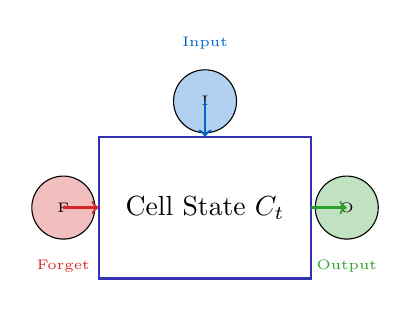
\begin{tikzpicture}[scale=0.9]
                % Memory cell
                \draw[thick, mlpurple] (0,0) rectangle (3,2);
                \node at (1.5, 1) {Cell State $C_t$};

                % Three gates
                \node[draw, circle, fill=mlred!30, minimum size=0.8cm] at (-0.5, 1) {\tiny F};
                \node[below, font=\tiny, mlred] at (-0.5, 0.4) {Forget};

                \node[draw, circle, fill=mlblue!30, minimum size=0.8cm] at (1.5, 2.5) {\tiny I};
                \node[above, font=\tiny, mlblue] at (1.5, 3.1) {Input};

                \node[draw, circle, fill=mlgreen!30, minimum size=0.8cm] at (3.5, 1) {\tiny O};
                \node[below, font=\tiny, mlgreen] at (3.5, 0.4) {Output};

                % Arrows
                \draw[->, thick, mlred] (-0.5, 1) -- (0, 1);
                \draw[->, thick, mlblue] (1.5, 2.5) -- (1.5, 2);
                \draw[->, thick, mlgreen] (3, 1) -- (3.5, 1);
            \end{tikzpicture}
            \end{center}

            \vspace{1em}
            \textbf{How Gates Work:}

            \begin{enumerate}
                \item \textcolor{mlred}{\textbf{Forget Gate:}} ``Remove outdated info''

                $f_t = \sigma(\ldots)$ (0 = forget all, 1 = keep all)

                \item \textcolor{mlblue}{\textbf{Input Gate:}} ``Add new important info''

                $i_t = \sigma(\ldots)$ (0 = ignore, 1 = add fully)

                \item \textcolor{mlgreen}{\textbf{Output Gate:}} ``Show relevant info''

                $o_t = \sigma(\ldots)$ (0 = hide, 1 = show)
            \end{enumerate}

            \vspace{1em}
            \textbf{Result:} Memory $C_t$ can persist for 100+ steps!
        \end{column}
    \end{columns}

    \bottomnote{Addition (not multiplication) + Gates (control) = Long-term memory preserved!}
\end{frame}

% Slide 15: LSTM Preview
\begin{frame}{Preview: LSTM (Long Short-Term Memory)}
    \begin{center}
    \includegraphics[width=0.75\textwidth]{../figures/lstm_gates_simple_bsc.pdf}
    \end{center}

    \vspace{-0.5em}
    \begin{columns}[T]
        \begin{column}{0.48\textwidth}
            \textbf{The LSTM Solution:}

            \vspace{0.5em}
            Two memory streams:

            \begin{enumerate}
                \item \textbf{Cell State $C_t$:} Protected long-term memory

                $C_t = \textcolor{mlred}{f_t} \odot C_{t-1} + \textcolor{mlblue}{i_t} \odot \tilde{C}_t$

                (Forget old + Add new)

                \item \textbf{Hidden State $h_t$:} Working memory

                $h_t = \textcolor{mlgreen}{o_t} \odot \tanh(C_t)$

                (Output from cell state)
            \end{enumerate}

            \vspace{1em}
            \textbf{Key Innovation:}

            Cell state $C_t$ uses \textcolor{mlgreen}{addition}, not multiplication!

            $\rightarrow$ Gradients flow unchanged through time

            $\rightarrow$ Can learn dependencies 100+ steps back!

            \vspace{1em}
            \textbf{Performance:}

            \begin{tabular}{l|c|c}
                Sequence Length & RNN & LSTM \\
                \hline
                10 words & 90\% & 92\% \\
                30 words & 45\% & 88\% \\
                100 words & 30\% & 85\% \\
            \end{tabular}
        \end{column}

        \begin{column}{0.48\textwidth}
            \begin{checkpoint}[Breakthrough Comparison]
            \textbf{Question:} What's the key difference between RNN and LSTM?

            \vspace{0.5em}
            \textbf{RNN Memory Update:}

            $h_t = \tanh(W_x x_t + W_h h_{t-1} + b)$

            \textcolor{mlred}{Multiplication at each step}

            \textcolor{mlred}{Gradient: $0.5^{20} \approx 0$}

            \vspace{1em}
            \textbf{LSTM Memory Update:}

            $C_t = f_t \odot C_{t-1} + i_t \odot \tilde{C}_t$

            \textcolor{mlgreen}{Addition preserves info}

            \textcolor{mlgreen}{Gradient: $\approx 1$ through cell state}

            \vspace{0.5em}
            This is the breakthrough!
            \end{checkpoint}

            \vspace{1em}
            \textbf{Example Success:}

            ``The \textcolor{mlblue}{cat} that ate the fish was hungry''

            LSTM keeps ``cat'' in $C_t$ for 10 steps

            Correctly predicts ``was'' (singular)

            \vspace{0.5em}
            RNN would have forgotten ``cat'' by step 10!
        \end{column}
    \end{columns}

    \bottomnote{LSTM solves vanishing gradient - enables true long-term dependencies}
\end{frame}

% Slide 16: Bridge to LSTM Slides
\begin{frame}{Next: Deep Dive into LSTM}
    \begin{columns}[T]
        \begin{column}{0.48\textwidth}
            \textbf{What You Learned Today (RNN):}

            \vspace{0.5em}
            \begin{enumerate}
                \item \textbf{The Challenge:} Variable-length sequences
                \item \textbf{RNN Insight:} Memory through recurrence
                \item \textbf{RNN Success:} Works for short sequences (5-10)
                \item \textbf{RNN Failure:} Vanishing gradient kills long memory
                \item \textbf{Root Cause:} Repeated multiplication
                \item \textbf{Human Insight:} Selective, protected memory
                \item \textbf{LSTM Idea:} Gates + Addition = Long memory
            \end{enumerate}

            \vspace{1em}
            \begin{realworld}[Where RNNs Still Used]
            Despite limitations, RNNs work well for:
            \begin{itemize}
                \item \textbf{Short sequences:} 5-15 steps
                \item \textbf{Real-time audio:} Low latency needed
                \item \textbf{Simple patterns:} Limited context required
                \item \textbf{Embedded systems:} Memory constraints
            \end{itemize}
            \end{realworld}
        \end{column}

        \begin{column}{0.48\textwidth}
            \textbf{What's Next (LSTM Slides):}

            \vspace{0.5em}
            \begin{enumerate}
                \item \textbf{Water Tank Analogy:} Concrete intuition for gates
                \item \textbf{Gate Mechanics:} How forget/input/output gates work
                \item \textbf{Worked Examples:} Step-by-step LSTM processing
                \item \textbf{Vector Mathematics:} Full equations explained
                \item \textbf{Training Details:} BPTT through LSTM
                \item \textbf{Applications:} Where LSTMs excel
                \item \textbf{Implementation:} PyTorch code
            \end{enumerate}

            \vspace{1em}
            \begin{intuition}[The Learning Journey]
            \textbf{Today:} Discovered WHY we need better memory

            (Vanishing gradient problem)

            \vspace{0.5em}
            \textbf{LSTM Slides:} Learn HOW gates solve it

            (Discovery-based approach)

            \vspace{0.5em}
            \textbf{Lab:} Build your own LSTM

            (Hands-on implementation)
            \end{intuition}

            \vspace{1em}
            \textbf{Ready?} Let's dive into LSTM architecture!
        \end{column}
    \end{columns}

    \bottomnote{RNNs taught us the problem - LSTMs show us the solution}
\end{frame}

% ==================== ACT 4: SYNTHESIS ====================

% Slide 17: RNN Applications
\begin{frame}{Where RNNs Work Well Today}
    \begin{columns}[T]
        \begin{column}{0.48\textwidth}
            \textbf{Successful Applications:}

            \vspace{0.5em}
            \textbf{1. Short-Sequence Tasks}

            \begin{itemize}
                \item \textbf{Name prediction:} ``Joh'' → ``n''
                \item \textbf{Next character:} Autocomplete (5-10 chars)
                \item \textbf{Sentiment:} Short reviews (1-2 sentences)
                \item \textbf{Simple classification:} Fixed-length input
            \end{itemize}

            \vspace{1em}
            \textbf{2. Real-Time Systems}

            \begin{itemize}
                \item \textbf{Voice recognition:} Process audio frame-by-frame
                \item \textbf{Gesture detection:} Short movement sequences
                \item \textbf{Sensor data:} Last 10 readings for prediction
            \end{itemize}

            \vspace{1em}
            \textbf{3. When Speed Matters}

            \begin{itemize}
                \item RNN: Simpler, faster than LSTM
                \item Fewer parameters to train
                \item Good for resource-constrained devices
            \end{itemize}
        \end{column}

        \begin{column}{0.48\textwidth}
            \textbf{Application Comparison:}

            \vspace{0.5em}
            \begin{center}
            \includegraphics[width=0.9\textwidth]{../figures/rnn_applications_bsc.pdf}
            \end{center}

            \vspace{1em}
            \textbf{Limitations Summary:}

            \begin{tabular}{l|c}
                Task & Max Length \\
                \hline
                Character prediction & 10-15 \\
                Sentiment (sentence) & 15-20 \\
                Short translation & 10-15 \\
                Paragraph understanding & \textcolor{mlred}{FAILS} \\
                Long document & \textcolor{mlred}{FAILS} \\
            \end{tabular}

            \vspace{1em}
            \begin{realworld}[Industry Use]
            \textbf{2010-2015:} RNNs everywhere

            \textbf{2015-2020:} LSTM replaces RNN for long sequences

            \textbf{2020+:} Transformers replace both

            \vspace{0.5em}
            But RNNs still used for simple, fast tasks!
            \end{realworld}
        \end{column}
    \end{columns}

    \bottomnote{RNNs: Great for short sequences, limited for long dependencies}
\end{frame}

% Slide 18: Summary
\begin{frame}{Summary: What We Learned About RNNs}
    \begin{columns}[T]
        \begin{column}{0.48\textwidth}
            \textbf{Key Concepts:}

            \vspace{0.5em}
            \begin{enumerate}
                \item \textbf{Sequential Data:} Order matters (text, speech, time series)

                \item \textbf{Traditional Networks Fail:} Fixed-size input, no memory

                \item \textbf{RNN Innovation:} Recurrent connections create memory

                $h_t = \tanh(W_x x_t + W_h h_{t-1} + b)$

                \item \textbf{Hidden State:} Carries context forward through time

                \item \textbf{Success:} Works well for short sequences (5-20 steps)

                \item \textbf{Failure:} Vanishing gradient for long sequences

                \item \textbf{Root Cause:} Repeated multiplication fades gradients

                $\text{gradient} \propto 0.5^{20} \approx 0$

                \item \textbf{Solution Preview:} LSTM uses addition + gates
            \end{enumerate}
        \end{column}

        \begin{column}{0.48\textwidth}
            \textbf{The Discovery Journey:}

            \vspace{0.5em}
            \begin{center}
            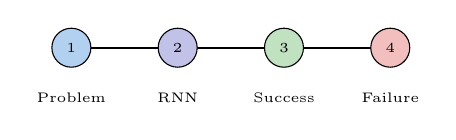
\begin{tikzpicture}[scale=0.9]
                % Timeline
                \draw[thick, ->] (0,0) -- (4.5,0);

                % Milestones
                \node[circle, draw, fill=mlblue!30] at (0,0) {\tiny 1};
                \node[below, font=\tiny] at (0,-0.5) {Problem};

                \node[circle, draw, fill=mlpurple!30] at (1.5,0) {\tiny 2};
                \node[below, font=\tiny] at (1.5,-0.5) {RNN};

                \node[circle, draw, fill=mlgreen!30] at (3,0) {\tiny 3};
                \node[below, font=\tiny] at (3,-0.5) {Success};

                \node[circle, draw, fill=mlred!30] at (4.5,0) {\tiny 4};
                \node[below, font=\tiny] at (4.5,-0.5) {Failure};
            \end{tikzpicture}
            \end{center}

            \vspace{1em}
            \textbf{Worked Examples Covered:}

            \begin{itemize}
                \item \textbf{Name prediction:} ``Joh'' → ``n''
                \item \textbf{Sentiment analysis:} Movie reviews
                \item \textbf{Long sentences:} Subject-verb agreement fails
            \end{itemize}

            \vspace{1em}
            \textbf{Mathematical Insights:}

            \begin{itemize}
                \item Recurrence creates memory
                \item Tanh activation bounds values
                \item Backpropagation through time (BPTT)
                \item Gradient vanishing from repeated multiplication
            \end{itemize}

            \vspace{1em}
            \begin{checkpoint}[Final Check]
            Can you explain why RNNs fail on long sequences?

            \textbf{Answer:} Vanishing gradient from repeated multiplication during backpropagation!
            \end{checkpoint}
        \end{column}
    \end{columns}

    \bottomnote{RNNs: First solution to variable-length sequences, but limited by vanishing gradient}
\end{frame}

% Slide 19: Next Steps
\begin{frame}{Next Steps: From RNN to LSTM}
    \begin{columns}[T]
        \begin{column}{0.48\textwidth}
            \textbf{Learning Path:}

            \vspace{0.5em}
            \begin{enumerate}
                \item \textbf{Today (RNN):} \textcolor{mlgreen}{[Completed]}

                \begin{itemize}
                    \item Understand sequential data challenge
                    \item Learn RNN architecture
                    \item Discover vanishing gradient problem
                \end{itemize}

                \item \textbf{Next (LSTM):} Continue reading

                \begin{itemize}
                    \item Discovery-based water tank analogy
                    \item Learn three gates (forget, input, output)
                    \item See how addition solves vanishing gradient
                    \item Worked examples with actual numbers
                \end{itemize}

                \item \textbf{Lab Session:} Hands-on implementation

                \begin{itemize}
                    \item Build RNN from scratch
                    \item Implement LSTM
                    \item Train on real text data
                    \item Compare performance
                \end{itemize}

                \item \textbf{Week 4 (Seq2seq):} Advanced architectures

                \begin{itemize}
                    \item Encoder-decoder models
                    \item Attention mechanism
                    \item Machine translation
                \end{itemize}
            \end{enumerate}
        \end{column}

        \begin{column}{0.48\textwidth}
            \textbf{Resources:}

            \vspace{0.5em}
            \textbf{Slides:}
            \begin{itemize}
                \item LSTM slides (next in sequence)
                \item Week 4: Seq2seq models
                \item Week 5: Transformers
            \end{itemize}

            \vspace{0.5em}
            \textbf{Labs:}
            \begin{itemize}
                \item Week 3 Lab: RNN/LSTM implementation
                \item Shakespeare generation notebook
                \item Sentiment classification exercise
            \end{itemize}

            \vspace{0.5em}
            \textbf{Code Examples:}
            \begin{itemize}
                \item PyTorch RNN tutorial
                \item Character-level generation
                \item Name prediction model
            \end{itemize}

            \vspace{1em}
            \textbf{Key Questions for Next Session:}

            \begin{enumerate}
                \item How do gates actually work? (Sigmoid functions)
                \item Why does addition preserve gradients? (Math proof)
                \item How to implement LSTM in PyTorch? (Code walkthrough)
                \item When to use RNN vs LSTM vs GRU? (Decision framework)
            \end{enumerate}

            \vspace{1em}
            \begin{center}
            \Large \textbf{Questions?}
            \end{center}
        \end{column}
    \end{columns}

    \bottomnote{Continue to LSTM slides for the complete solution to long-range dependencies}
\end{frame}

% ==================== APPENDIX: MATHEMATICAL DETAILS ====================

\appendix

% Appendix Slide 1: RNN Mathematics - Forward and Backward Pass
\begin{frame}{Appendix A: RNN Mathematics - Complete Equations}
    \begin{columns}[T]
        \begin{column}{0.48\textwidth}
            \textbf{Forward Pass (Inference):}

            \vspace{0.5em}
            At each time step $t = 1, 2, \ldots, T$:

            \vspace{0.5em}
            \textbf{1. Hidden state update:}
            \[
            h_t = \tanh(W_x x_t + W_h h_{t-1} + b_h)
            \]

            where:
            \begin{itemize}
                \item $x_t \in \mathbb{R}^{d_x}$: input at time $t$
                \item $h_t \in \mathbb{R}^{d_h}$: hidden state
                \item $W_x \in \mathbb{R}^{d_h \times d_x}$: input weight matrix
                \item $W_h \in \mathbb{R}^{d_h \times d_h}$: recurrent weight matrix
                \item $b_h \in \mathbb{R}^{d_h}$: hidden bias
            \end{itemize}

            \vspace{0.5em}
            \textbf{2. Output computation:}
            \[
            y_t = W_y h_t + b_y
            \]

            where:
            \begin{itemize}
                \item $W_y \in \mathbb{R}^{d_y \times d_h}$: output weight matrix
                \item $b_y \in \mathbb{R}^{d_y}$: output bias
            \end{itemize}

            \vspace{0.5em}
            \textbf{3. Probability distribution:}
            \[
            p(w_t \given w_{<t}) = \text{softmax}(y_t)
            \]

            where softmax: $\text{softmax}(z)_i = \frac{e^{z_i}}{\sum_j e^{z_j}}$
        \end{column}

        \begin{column}{0.48\textwidth}
            \textbf{Backward Pass (Training - BPTT):}

            \vspace{0.5em}
            \textbf{Loss function:}
            \[
            L = -\sum_{t=1}^{T} \log p(w_t^* \given w_{<t})
            \]

            where $w_t^*$ is the true next word.

            \vspace{0.5em}
            \textbf{Backpropagation through time (BPTT):}

            \vspace{0.5em}
            Output gradient:
            \[
            \frac{\partial L}{\partial y_t} = \hat{y}_t - y_t^*
            \]

            \vspace{0.5em}
            Hidden state gradient at time $t$:
            \[
            \frac{\partial L}{\partial h_t} = \frac{\partial L}{\partial y_t} \frac{\partial y_t}{\partial h_t} + \frac{\partial L}{\partial h_{t+1}} \frac{\partial h_{t+1}}{\partial h_t}
            \]

            \vspace{0.5em}
            Expanded:
            \[
            \frac{\partial L}{\partial h_t} = W_y^T \frac{\partial L}{\partial y_t} + W_h^T \frac{\partial L}{\partial h_{t+1}} \odot \tanh'(z_{t+1})
            \]

            where $z_t = W_x x_t + W_h h_{t-1} + b_h$

            \vspace{0.5em}
            \textbf{Weight gradients:}
            \[
            \frac{\partial L}{\partial W_x} = \sum_{t=1}^{T} \frac{\partial L}{\partial h_t} \odot \tanh'(z_t) \cdot x_t^T
            \]

            \[
            \frac{\partial L}{\partial W_h} = \sum_{t=1}^{T} \frac{\partial L}{\partial h_t} \odot \tanh'(z_t) \cdot h_{t-1}^T
            \]
        \end{column}
    \end{columns}

    \bottomnote{BPTT unrolls the network through time and accumulates gradients across all time steps}
\end{frame}

% Appendix Slide 2: Vanishing Gradient Mathematical Proof
\begin{frame}{Appendix B: Vanishing Gradient - Mathematical Derivation}
    \begin{columns}[T]
        \begin{column}{0.48\textwidth}
            \textbf{Gradient Flow Analysis:}

            \vspace{0.5em}
            To update weights based on early time steps, gradients must flow backward through all intermediate steps.

            \vspace{0.5em}
            \textbf{Chain rule for gradient at time $t$:}

            \[
            \frac{\partial L}{\partial h_t} = \frac{\partial L}{\partial h_T} \prod_{k=t+1}^{T} \frac{\partial h_k}{\partial h_{k-1}}
            \]

            \vspace{0.5em}
            \textbf{Jacobian of hidden state:}

            Recall: $h_t = \tanh(W_x x_t + W_h h_{t-1} + b_h)$

            \[
            \frac{\partial h_t}{\partial h_{t-1}} = \text{diag}(\tanh'(z_t)) \cdot W_h
            \]

            where $\tanh'(z) = 1 - \tanh^2(z)$

            \vspace{0.5em}
            \textbf{Product expansion:}

            \begin{align*}
            \frac{\partial L}{\partial h_t} &= \frac{\partial L}{\partial h_T} \prod_{k=t+1}^{T} \text{diag}(\tanh'(z_k)) \cdot W_h \\
            &= \frac{\partial L}{\partial h_T} \left( \prod_{k=t+1}^{T} \text{diag}(\tanh'(z_k)) \right) W_h^{T-t}
            \end{align*}

            \vspace{0.5em}
            \textbf{Key observation:} Product of $T-t$ matrices!
        \end{column}

        \begin{column}{0.48\textwidth}
            \textbf{Why Gradients Vanish:}

            \vspace{0.5em}
            \textbf{1. Tanh derivative bounds:}

            \[
            0 < \tanh'(z) = 1 - \tanh^2(z) \leq 1
            \]

            Typically: $\tanh'(z) \approx 0.2$ to $0.5$ for most $z$

            \vspace{0.5em}
            \textbf{2. Spectral radius of $W_h$:}

            Let $\lambda_{\max}$ be the largest eigenvalue of $W_h$.

            For gradient flow to be stable:
            \[
            \left\| \frac{\partial h_t}{\partial h_{t-1}} \right\| = \left\| \text{diag}(\tanh'(z_t)) W_h \right\| \lesssim 1
            \]

            \vspace{0.5em}
            \textbf{3. Long-term gradient magnitude:}

            \[
            \left\| \frac{\partial L}{\partial h_t} \right\| \approx \left\| \frac{\partial L}{\partial h_T} \right\| \cdot \gamma^{T-t}
            \]

            where $\gamma = \| \text{diag}(\tanh'(z)) W_h \|$

            \vspace{0.5em}
            \textbf{Typical case:} $\gamma \approx 0.5$

            \vspace{0.5em}
            For $T-t = 20$ steps back:
            \[
            \text{gradient magnitude} \approx 0.5^{20} \approx 9.5 \times 10^{-7}
            \]

            \textcolor{mlred}{\textbf{Vanished!}}

            \vspace{0.5em}
            \textbf{Consequence:} Early time steps contribute negligible gradient $\rightarrow$ cannot learn long-term dependencies.
        \end{column}
    \end{columns}

    \bottomnote{Solution: LSTM uses additive cell state updates to bypass multiplicative gradient decay}
\end{frame}

\end{document}
